\documentclass[doc,biblatex,apacite]{apa6}
\usepackage{array}
\usepackage{float}
\usepackage{graphicx}
\usepackage[american]{babel}
\usepackage{amsmath}
\usepackage{comment}
\usepackage{multirow}
\usepackage{breqn}
\usepackage{rotating}
\usepackage{pdflscape}
\usepackage{listings}
\usepackage{caption}
\usepackage{subcaption}
\usepackage{alltt}




\author{Yi Chen}
\affiliation{Teachers College, Columbia University}
\title{Linear Model and Experimental Design}
\abstract{ In this document, I will present my answer for the task 1 questions for Linear Model and Experimental Design.
}

\keywords{OLS Regression Diagnostics}

\begin{document}
\maketitle

\section{Task 1}

The model for this task can be described as,

\begin{equation} \label{eq1}
    \begin{split}
        Murder = \beta_0 + \beta_1 Population + \beta_2 Income + \beta_3 Illiteracy  \\
        + \beta_4 Life.Exp + \beta_5 HS.Grad + \beta_6 Frost + \beta_7 Area + \epsilon
    \end{split}
    \end{equation}


The estimated value of the parameters are: $\hat{\beta_0}=1.222e+02$, $\hat{\beta_1}=1.880e-04$, $\hat{\beta_2}=-1.592e-04$, $\hat{\beta_3}=1.373$,$\hat{\beta_4}=-1.655$, $\hat{\beta_5}=3.234e-02$, $\hat{\beta_6}= -1.288e-02$, and $\hat{\beta_7} = 5.967e-06$.
$R^2 = 80.83\%$, Residual standard error is 1.746 on 42 degrees of freedom.

This result means, the predictors in the model can explain the 80.83 \% variance in the murder rate. The standard residuals explain the standardized deviance between estimated value and the observed value. 
The estimated intercept value indicates the expected murder rate when all the predictors setting the value as 0, which is unrealistic.
Take the coefficient estimated value of Life.Exp for example, it means if we take all the other predictors' value as fixed, when we increases the value of Life.Exp in 1 unit, the murder rate will decrease  -1.655 unit.
The estimated value is very different. 
In order to increase the comparability of the estimated value, we should do the standardization among the predictors in advance.


\section{Task 2}

High leverage: hat-value measures the distance from that point to the mean of the predictor variable. It is the
Mahalanobis distance.

High Inference: Cook’s distance is a measure of the influence of a point. It may be though of as a measure that takes
the product of a point’s discrepancy and its leverage

\section{Task 3}

The influence plot is shown in the Figure 1.
Nevada has the highest studentized residual, Alaska has the highest leverage (hat value), and Alaska has the highest inference (Cook’s distance)
\begin{figure}
    \centering
    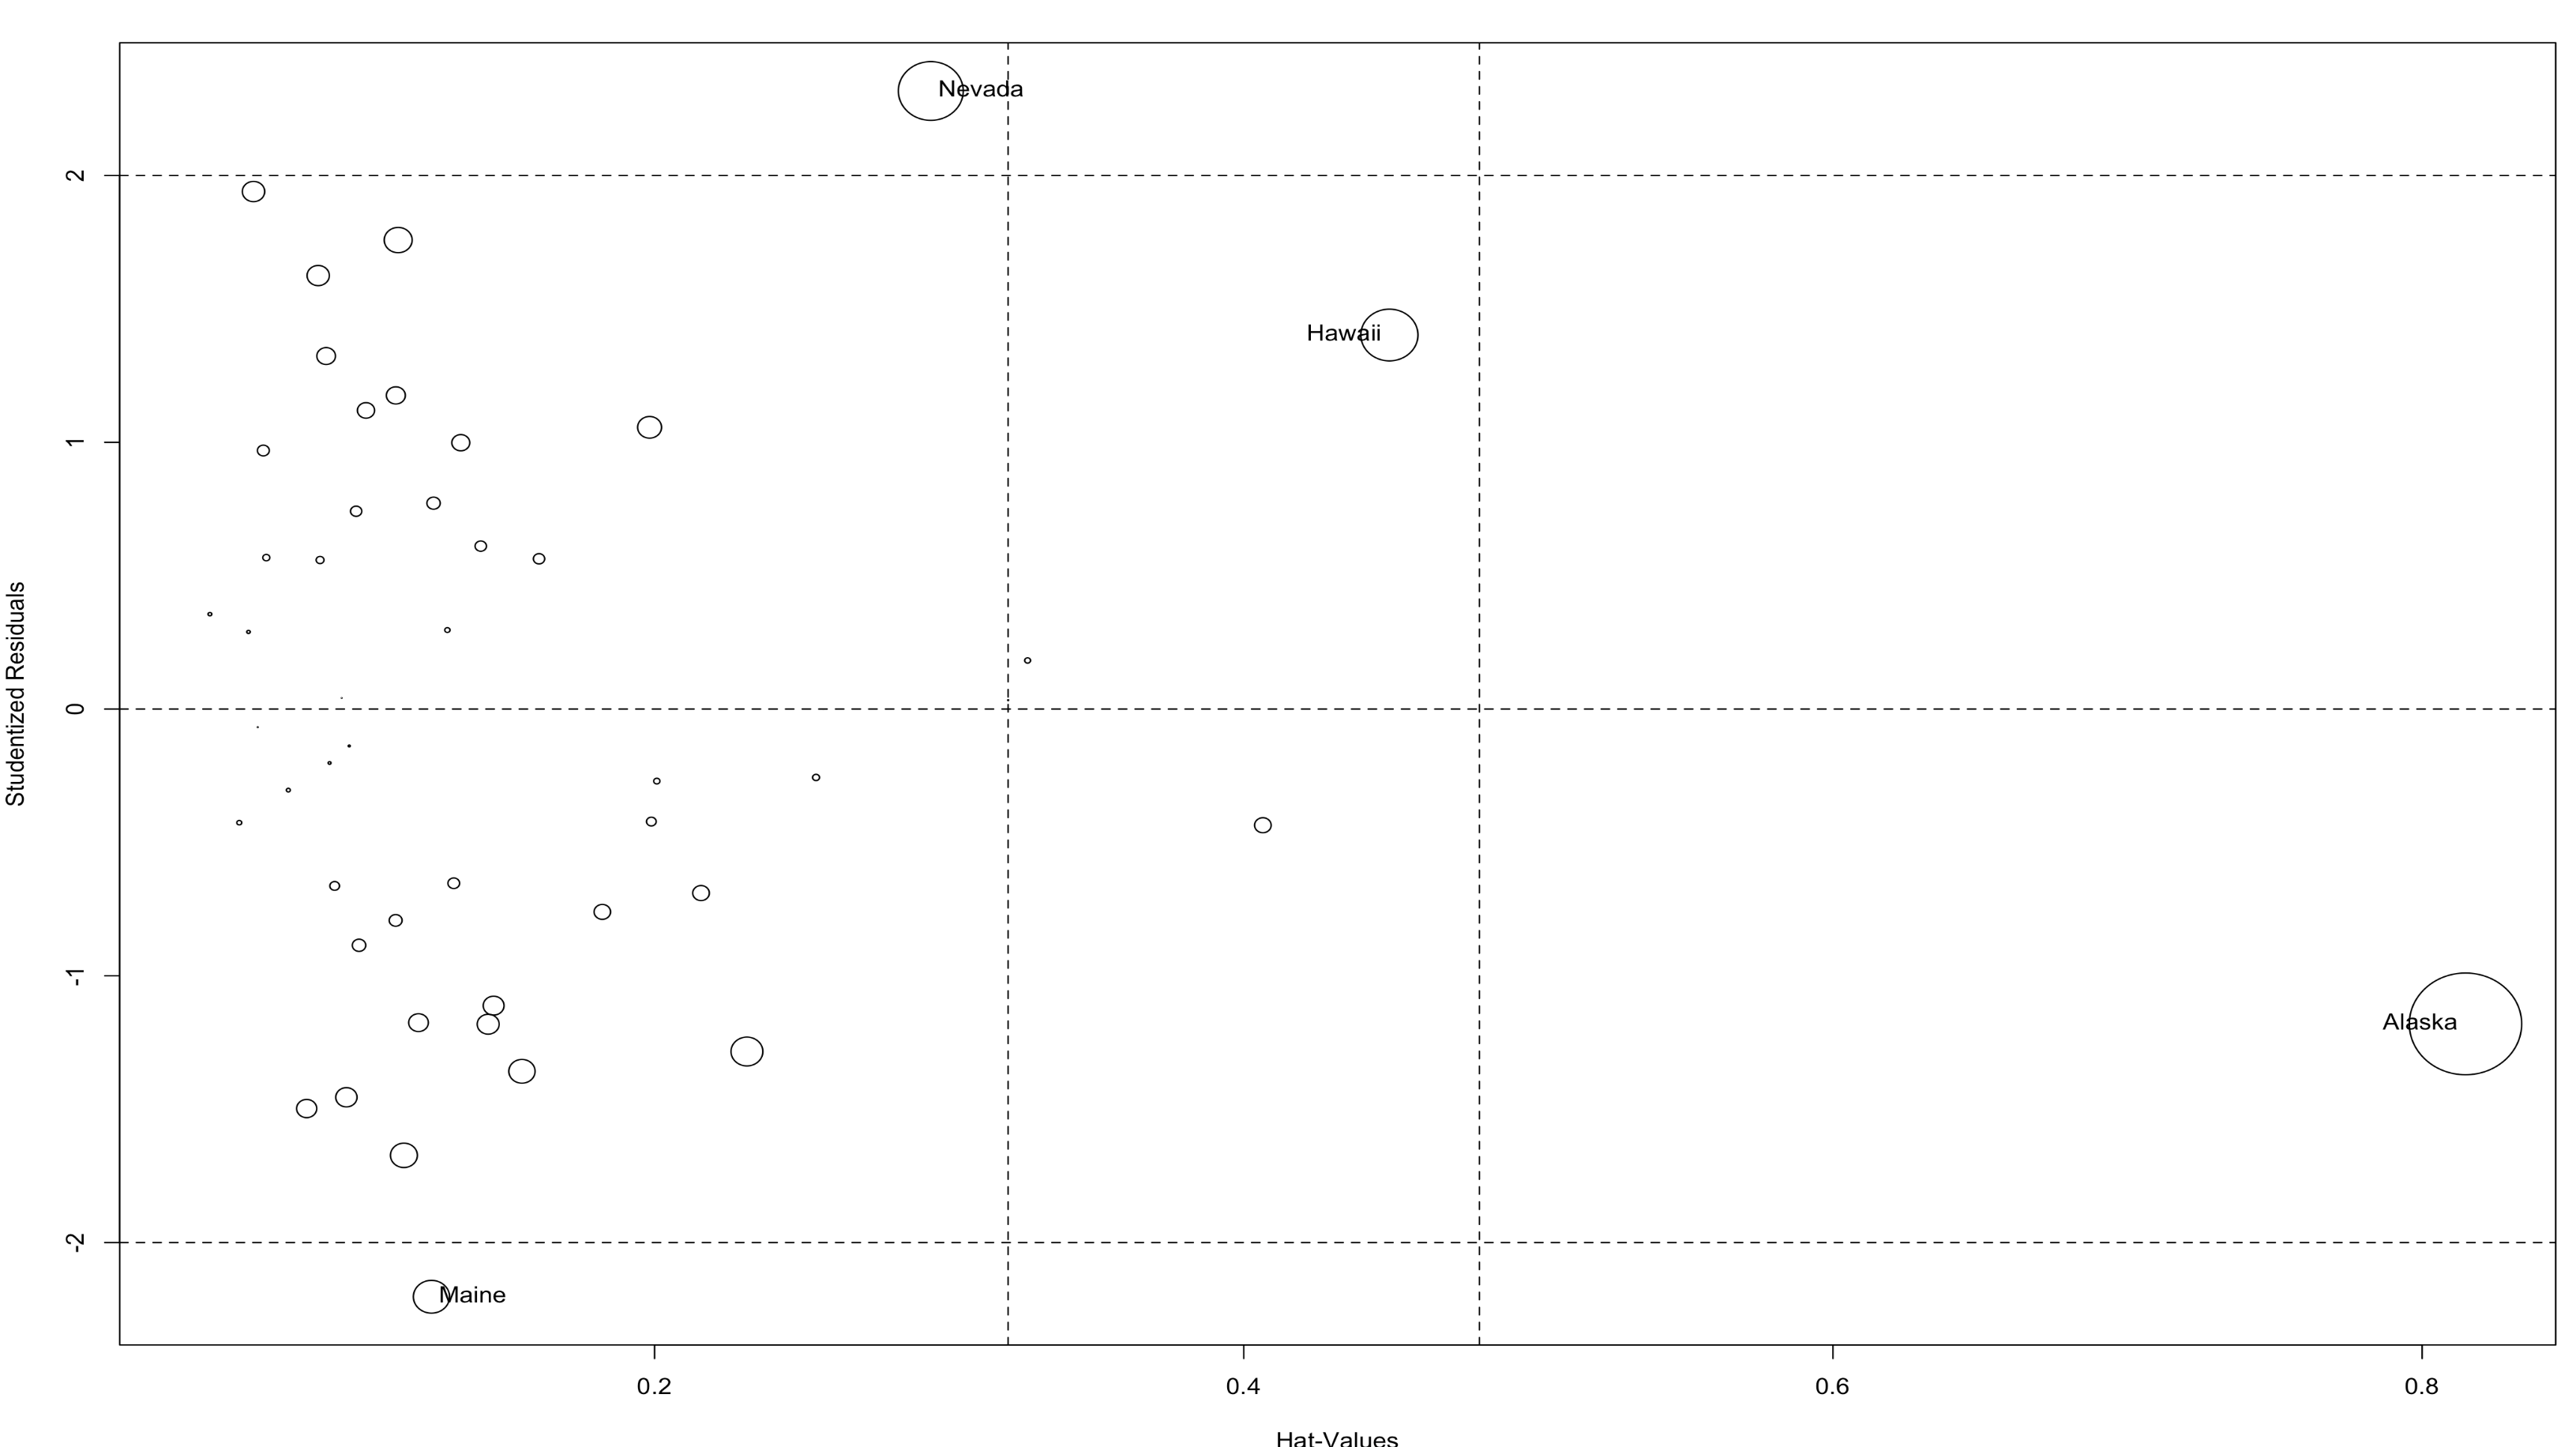
\includegraphics[width=10cm]{influence_plot.png}
    \caption{Influence Plot}
\end{figure}


\section{Task 4}
Personally, I do not think we should delete the data for Alaska. 

\begin{enumerate}
    \item The social and economic condition for Alaska is very different with other states in USA, which explain why their data is outliers. 
    These data does not have obvious error or human-made mistakes. 
    If the research is about the whole USA, Alaska and other places like Hawaii should all be included. 
    \item We should standardize the predictors before fitting the model. The result may be different.
    \item If necessary, just run two different analyses with and without Alaska.
    
\end{enumerate}

\section{Task 5}
The QQ plot of the studentized residuals is shown in the Figure 2.
\begin{figure}
    \centering
    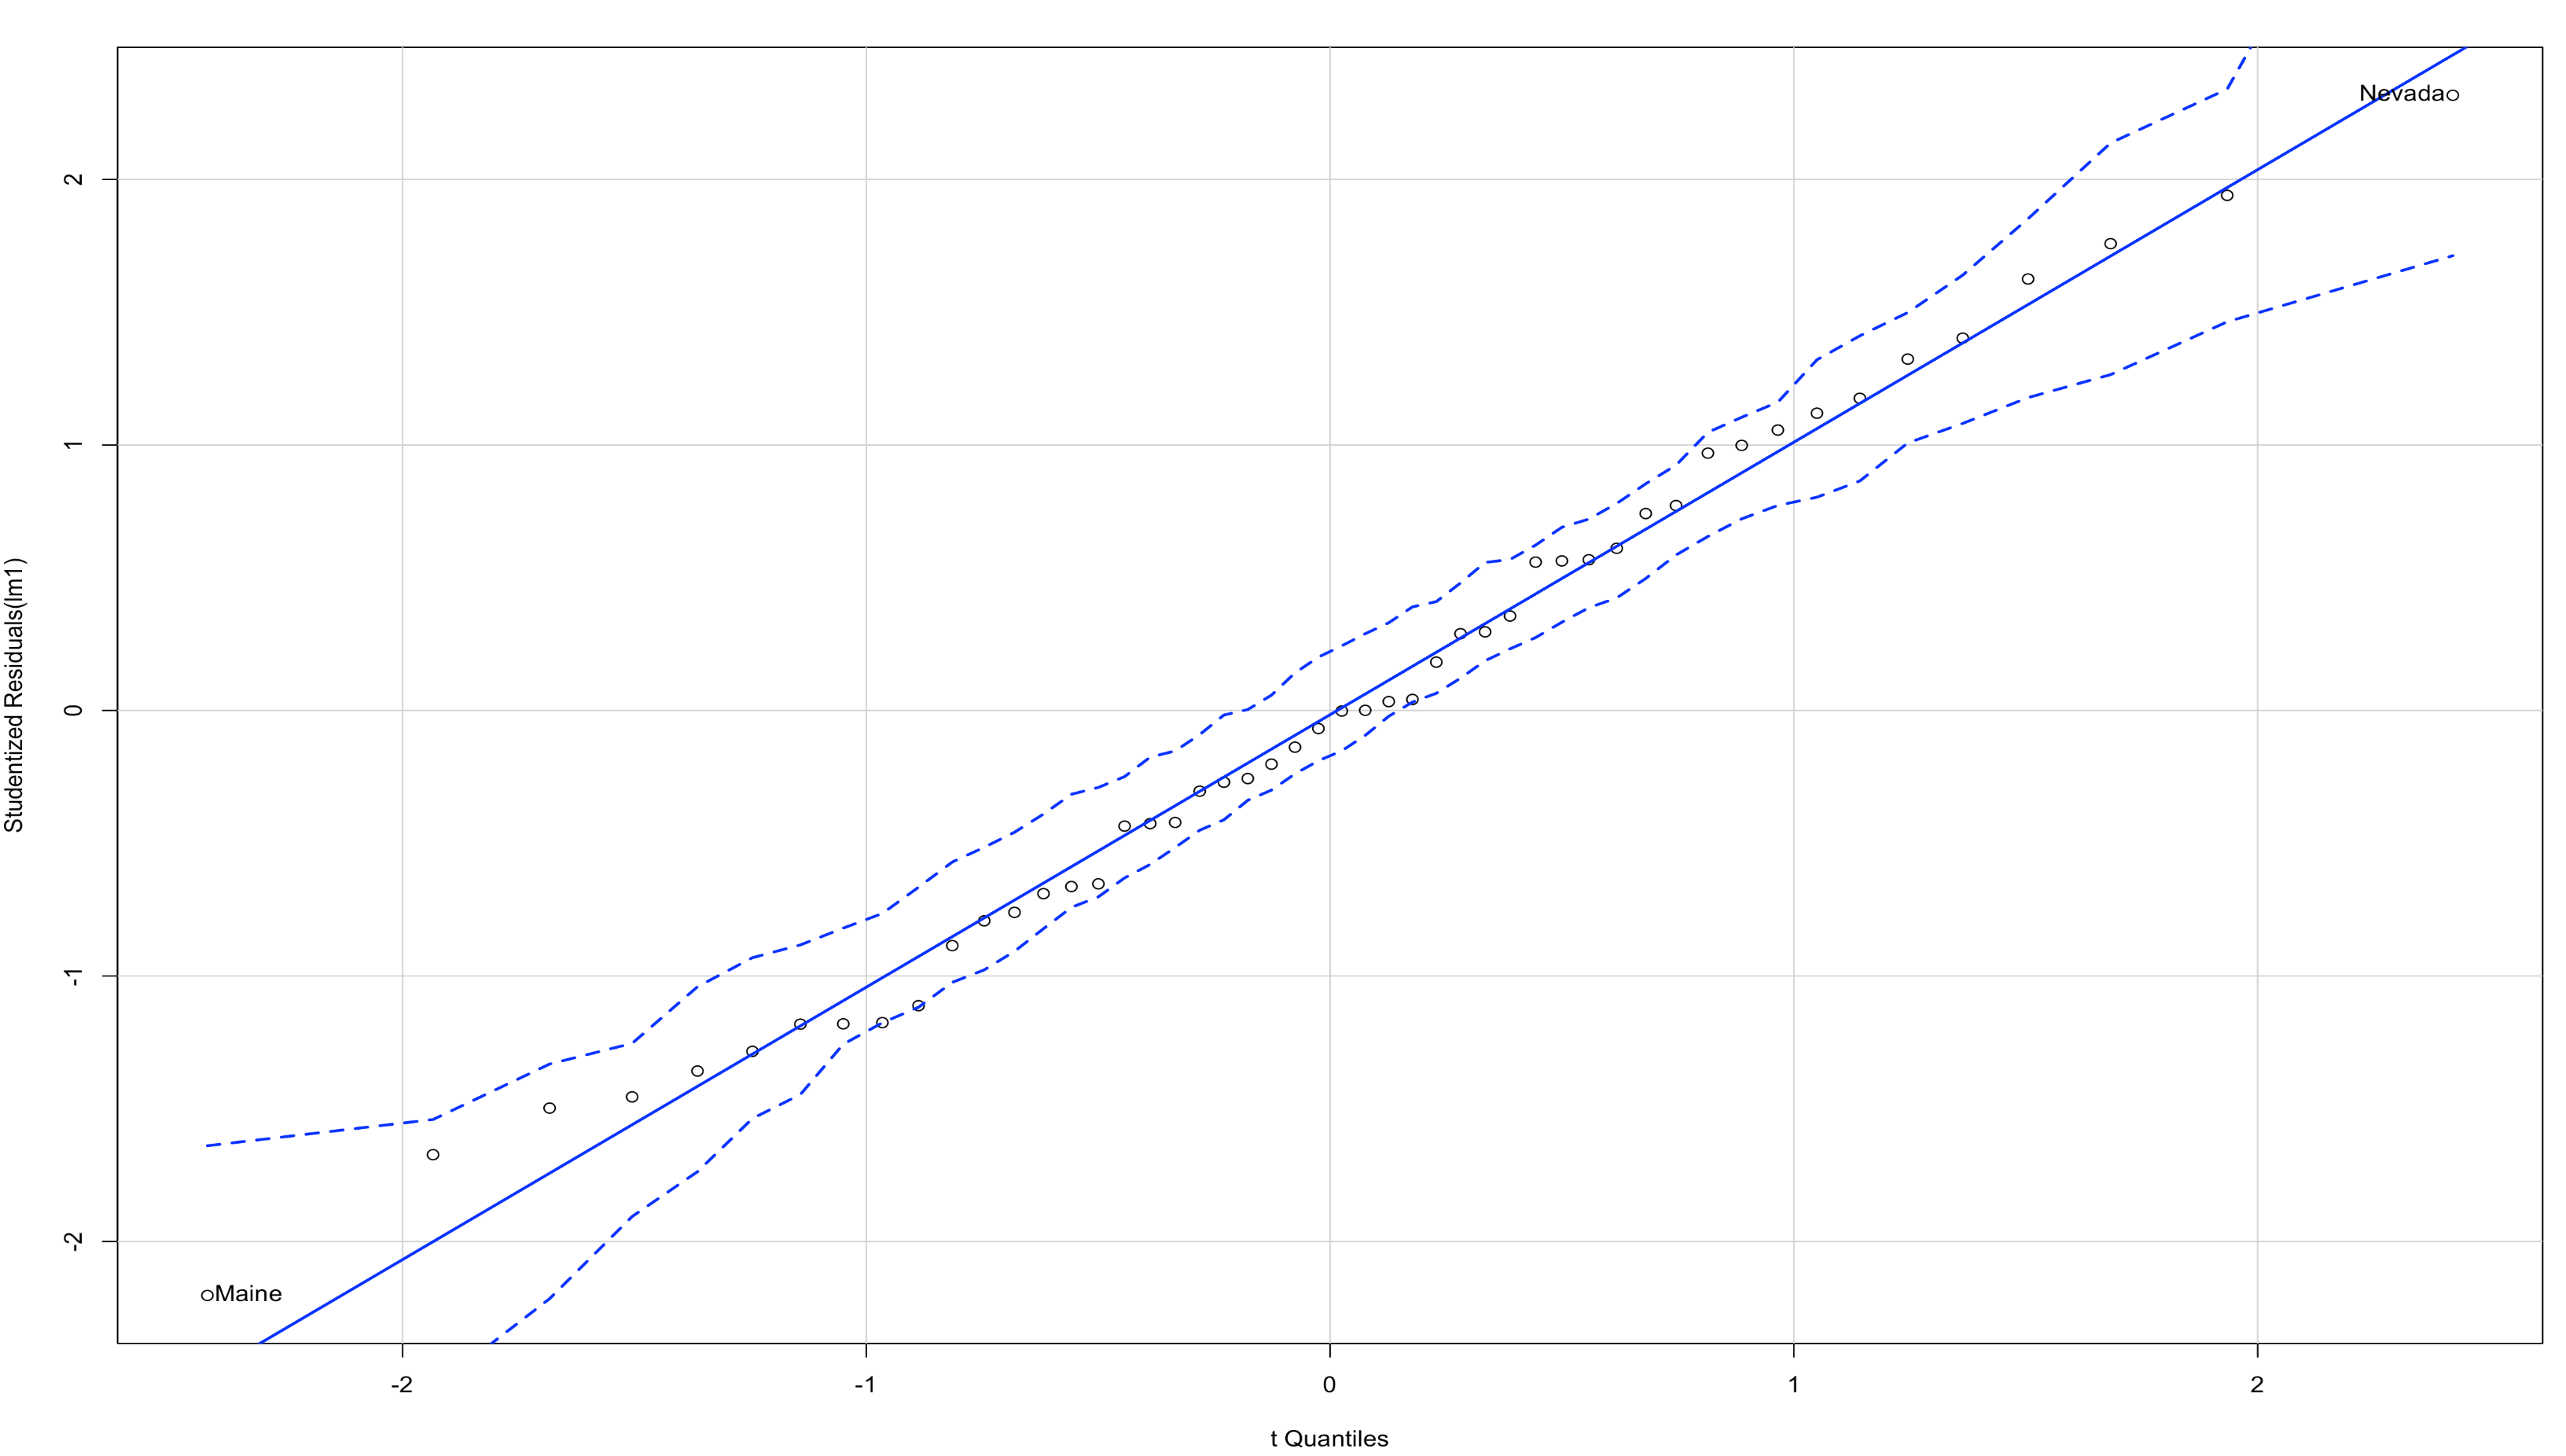
\includegraphics[width=10cm]{qqplot.png}
    \caption{QQ Plot}
\end{figure}

If the observed studentized residuals really follows the t distribution, the points should be close to the 45 degree line.
Based on the evidence that all points are in the 96\% confidence interval, we can claim that the normality assumption is hold.


\section{Task 6}
The plot of studentized residuals against the ordered fitted is shown in the Figure 3.

\begin{figure}
    \centering
    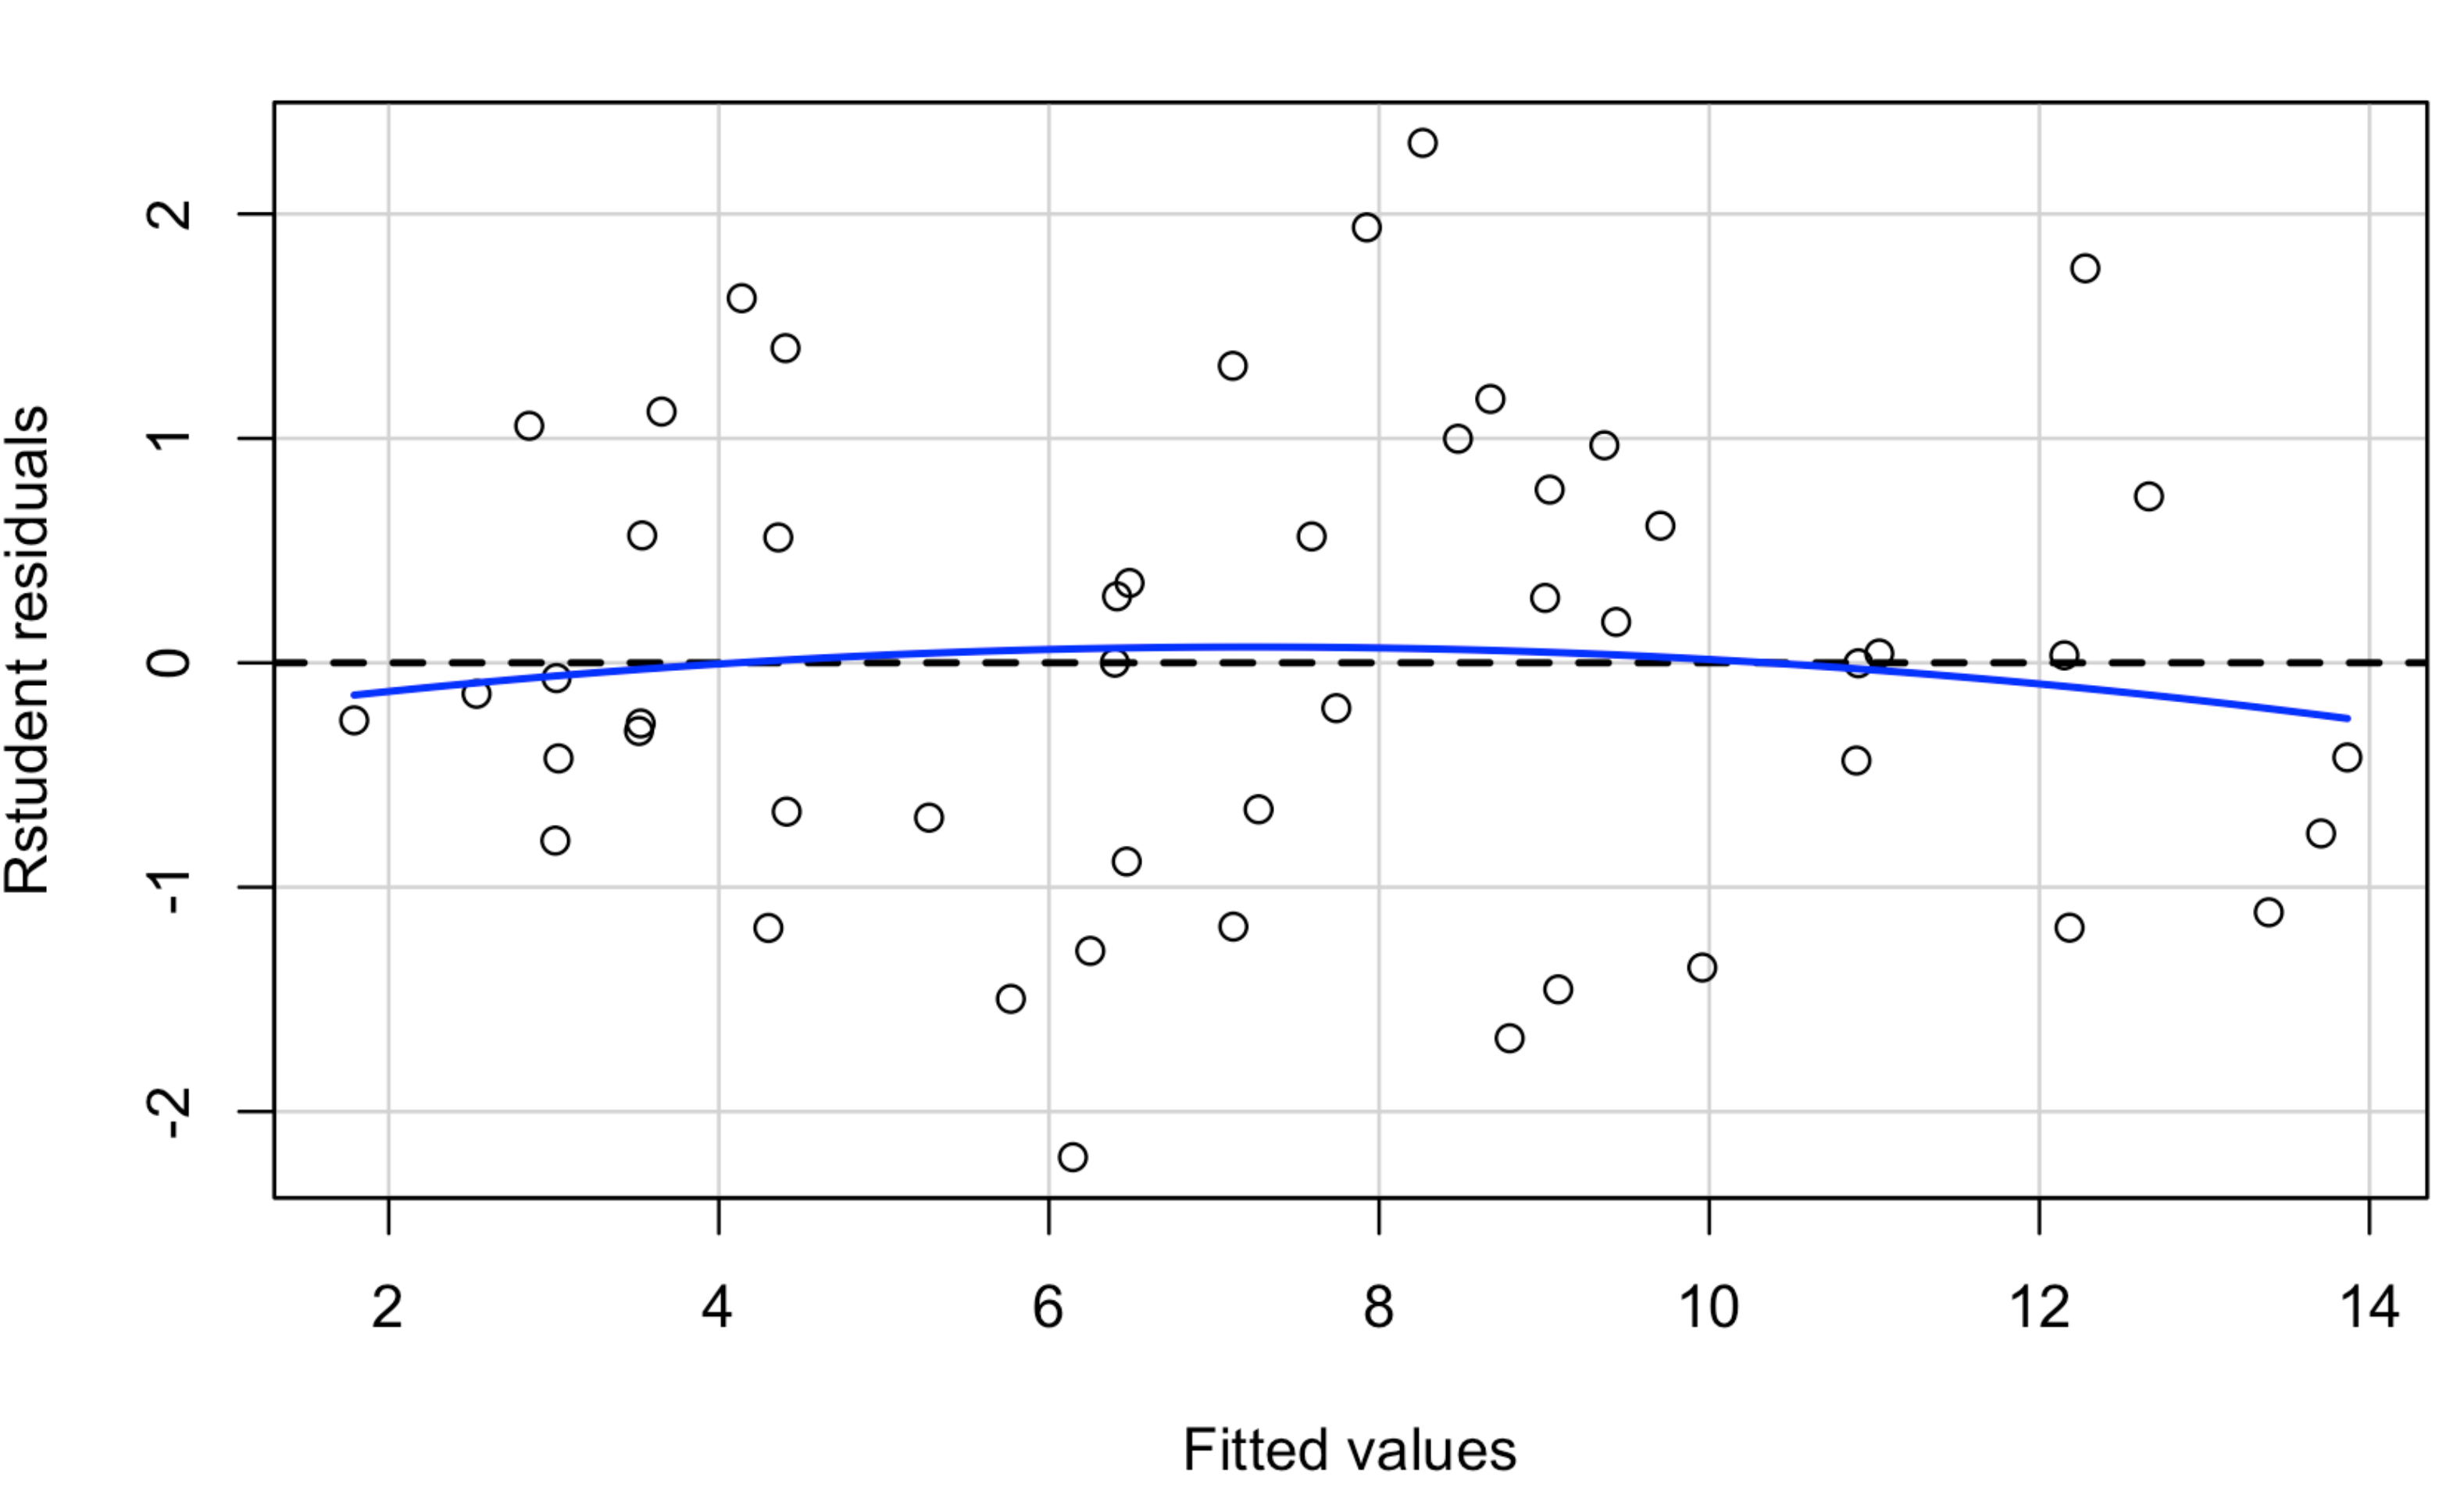
\includegraphics[width=10cm]{residual_plot.png}
    \caption{Residuals against Fitted Value Plot}
\end{figure}

Generally speaking, the error variance is constant. 
There is only a slight bigger variance when the fitted value is
between 6 and 10, but it is not obvious.

\section{Task 7}
The CR plot for the 7 predictors are shown in the Figure 4.
\begin{figure}
    \centering
    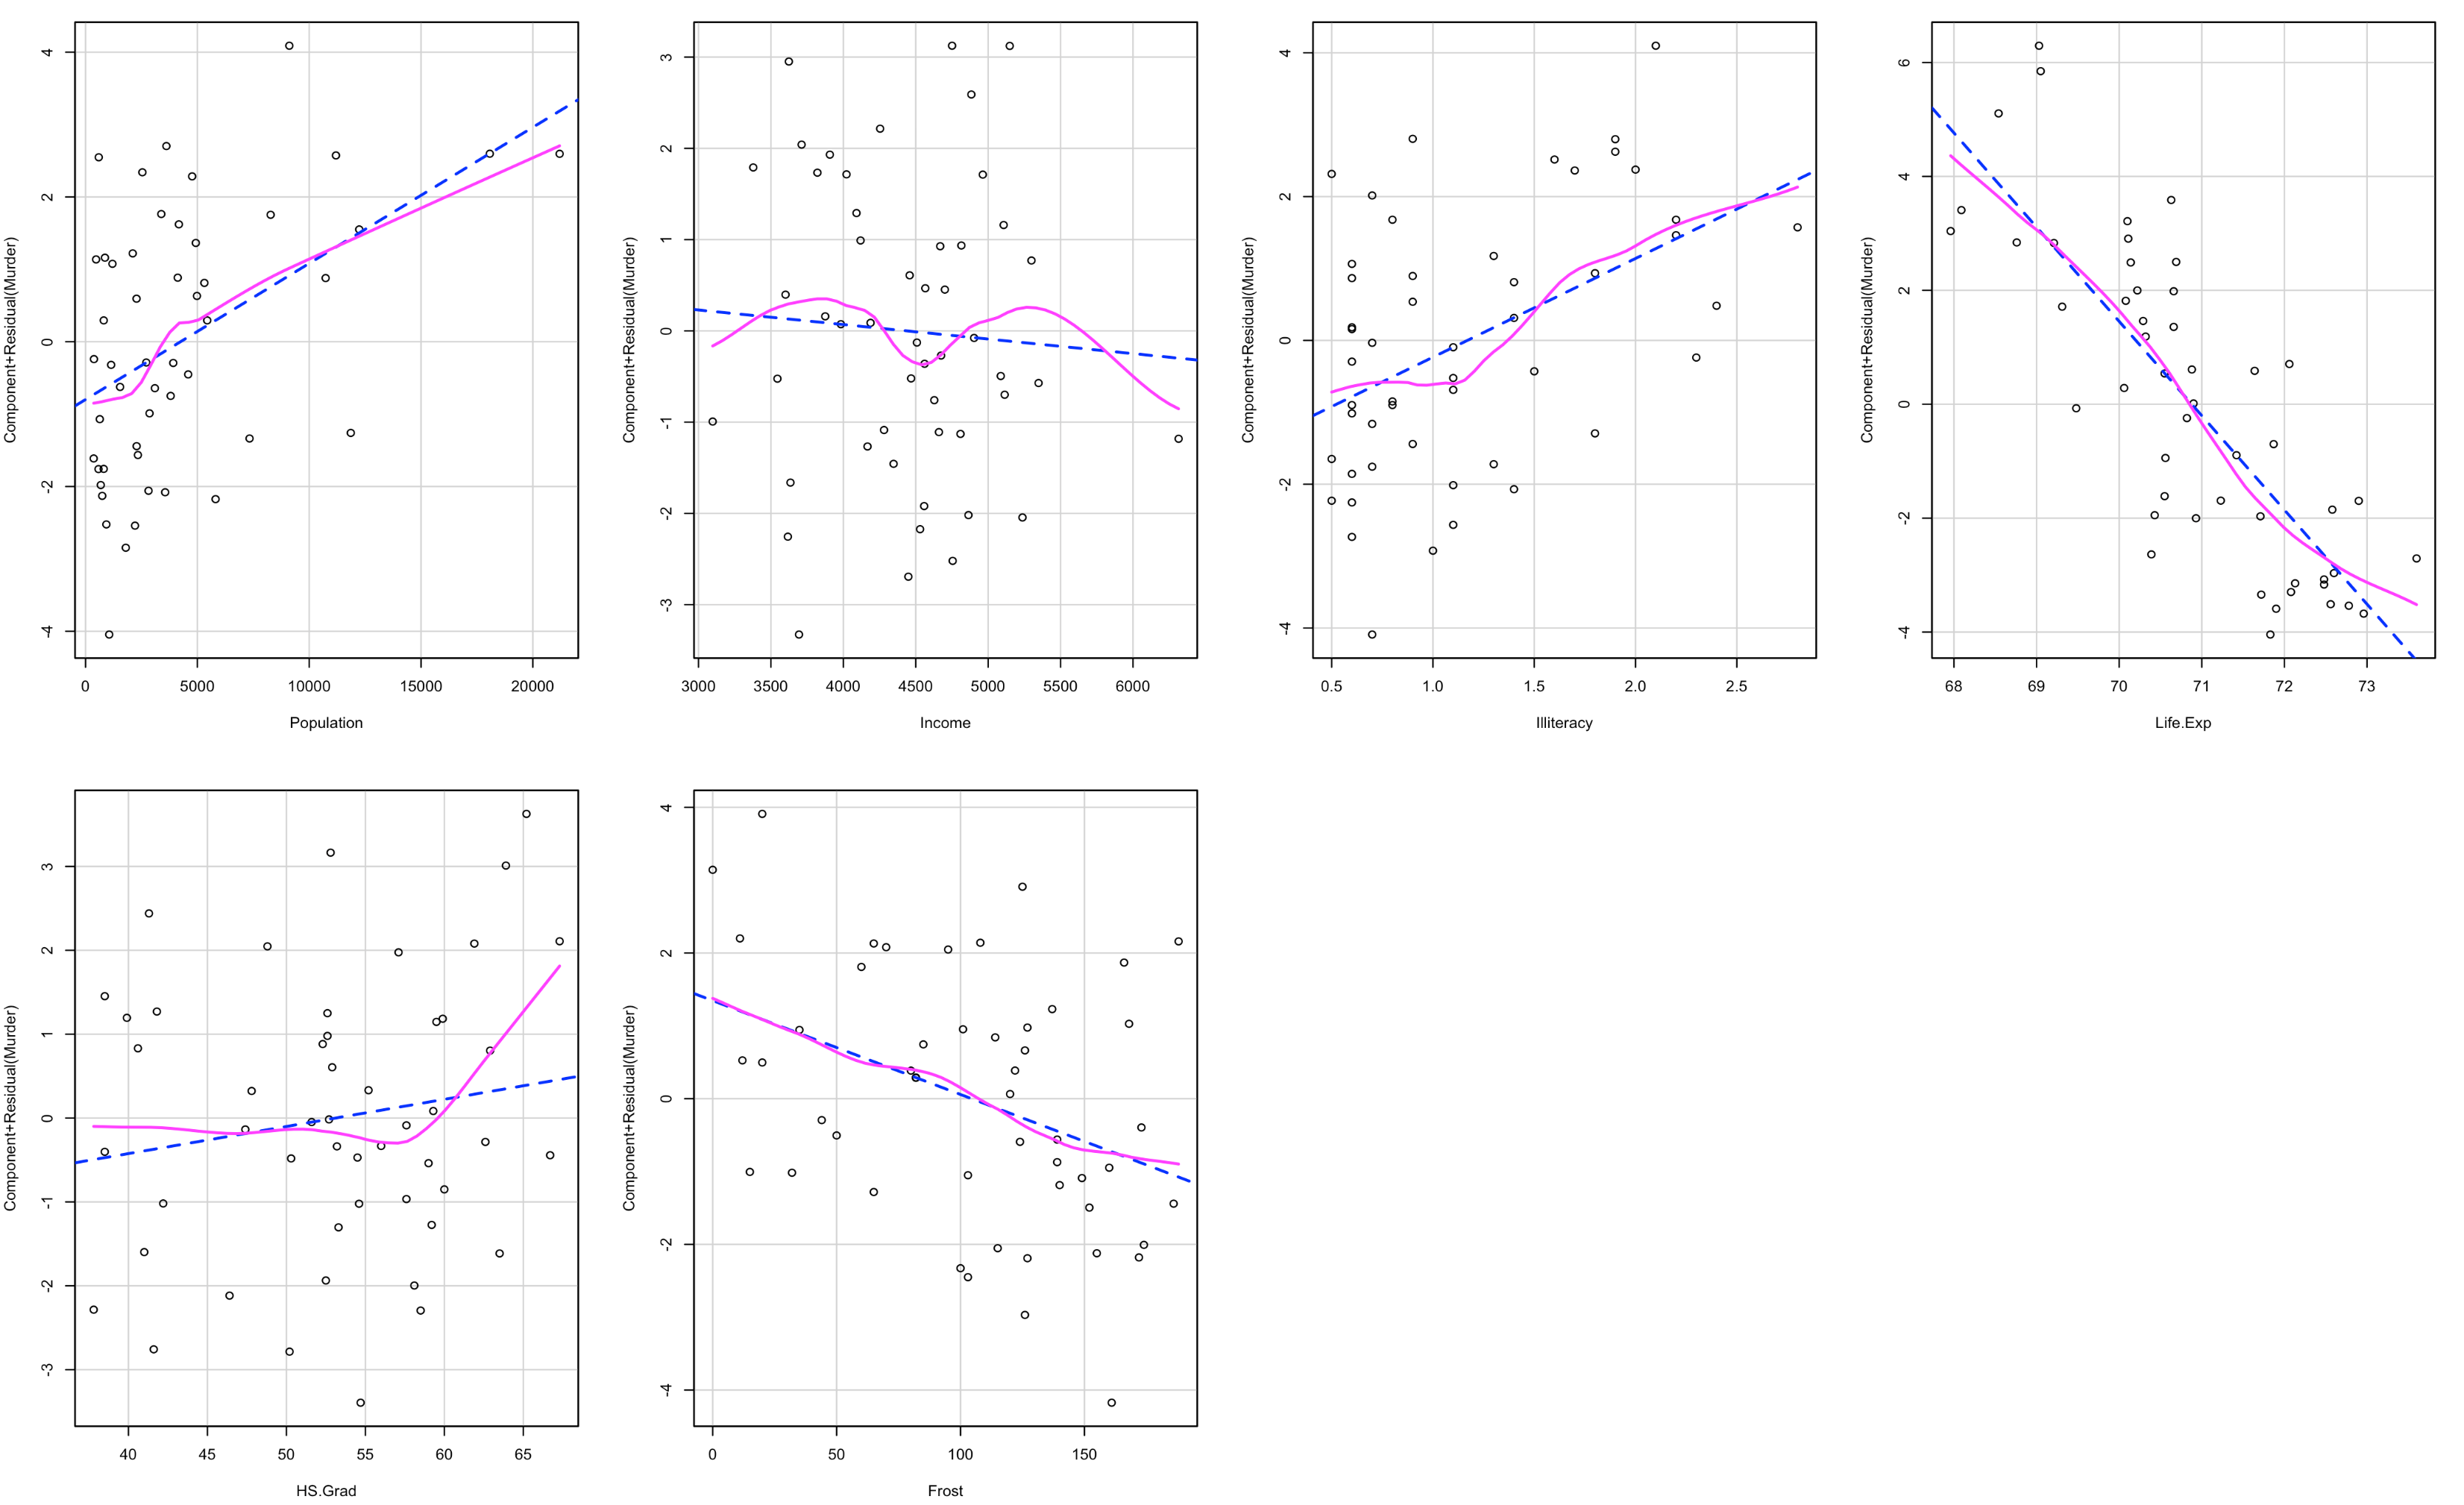
\includegraphics[width=10cm]{CRPLot.png}
    \caption{CR Plot}
\end{figure}

The non-parametric regression and OLS regression lines are close for almost all 7 variables. 
For area, income the non-linearity, and HS.Grad the non-linearity is a little violated.
It would be better to do some transformation of these variable before regression.
Generally speaking, the linearity assumption is hold.

\section{Task 8}
According the the pairwise correlation between different variables, there is no clear linear correlation between predictors.
All variable have relatively small VIF which means there is no clear multicollinearity.
The variable with the biggest VIF is "Illiteracy" with the variable as 4.135956.
The $R_{j}$ square value is calculated by make the "Illiteracy" as the outcome variable and all other original predictors as the predictors. 
The corresponding $R^2$ is the $R_{j}$ square value.
The $R_{j}$ value for "Illiteracy" is 75.82 \%.


\end{document}
